\DiaryEntry{Expected Distance between random Points on the Unit-sphere}{2018-08-03}{Maths}


We can generate random points uniformly on the unit sphere using \href{https://stats.stackexchange.com/questions/7977/how-to-generate-uniformly-distributed-points-on-the-surface-of-the-3-d-unit-sphe}{this link}

\subsection{2-dimensional case}

Fix one point $A = (1,0)$ and choose the other one $B$ randomly: $B = (x, \sqrt{1-x^2})$. The distance $d$ between the two is

\bee
d^2 = (1-x)^2 + 1 - x^2 = 2(1-x)
\eee

In the 2-dimensional case $x$ is \emph{not} distributed uniformly, however $x = \cos \phi$ and $\phi$ is distributed uniformly on the interval $[0, 2\pi]$. Therefore, the expected values for $d^2$ and $d$ become

\bee
\mE(d^2) = \frac{1}{2 \pi} \int_0^{2\pi} 2(1-\cos \phi)d\phi = \cdots = 2
\eee

and

\bee
\mE(d) = \frac{1}{2 \pi} \int_0^{2\pi} \sqrt{2(1-\cos \phi)} d\phi = \cdots = \frac{4}{\pi}
\eee

respectively.

\subsection{3-dimensional Case}

We proceed in a similar manner, fixing $A = (1,0,0)$ and choosing $B$ randomly: $B = (x,y,z)$. The distance $d^2$ then becomes

\bee
d^2 = (1-x)^2 + y^2 + z^2 = (1-x)^2 + 1 - x^2 = 2(1-x)
\eee

where we have used that the point $B$ is on the unit-sphere; i.e. $x^2 + y^2 + z^2 = 1$. According to the \href{http://mathworld.wolfram.com/ArchimedesHat-BoxTheorem.html}{Archimedes hat theorem}, $x$ is distributed uniformly on $[-1,1]$, and we have the following expected values of $d^2$ and $d$

\bee
\mE(d^2) = \frac{1}{2} \int_{-1}^{1} 2(1-x)dx = \cdots = 2
\eee

and

\bee
\mE(d) = \frac{1}{2} \int_{-1}^{1} \sqrt{2(1-x)} dx = \cdots = \frac{4}{3}
\eee

respectively.

\subsection{Higher Dimensions}

For $D > 3$, the expression for $d$ stays the same,

\be\label{2018-08-03:eqgen}
d^2 = (1-x_1)^2 + x_2^2 + x_3^2 + \cdots x_D^2 = (1-x_1)^2 + 1 - x_1^2 = 2(1-x_1)
\ee

because we have used the generalized unit sphere definition $\sum_k x_k^2 = 1$. However, $x$ has a \emph{different} distribution anymore, and therefore above calculation does not work.

The coordinate $x_1$ is given as

\bee
x_1 = \frac{X_1}{\sqrt{X_1^2 + X_2^2 + \cdots + X_D^2}}
\eee

where $X_D \sim \Nc(0,1)$. \todo{How can we derive the following empirical results?}

Empirically (Julia), the distribution of $d^2$ looks Gaussian with mean $2$. However, this is not really true, as $d^2$ must be larger than $0$ and - choosing the "worst case" $x_1 = -1$ - smaller than $4$ (check with \eqref{2018-08-03:eqgen}). The following Figure shows a histogram for $D = 10$.

\begin{figure}[H]
	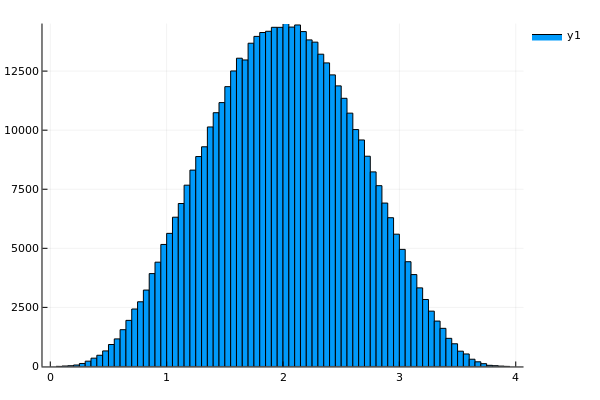
\includegraphics[scale=0.65]{images/distance_point_sphere_1.png}
\end{figure}

For larger $D$, the distribution becomes more centered around $d^2 = 2$.

Next we investigate the angle between the vector $0A$ (connecting the zero point $(0,\ldots,0)$ with $A = (1,0,\ldots,0)$) and $0B$ (connecting the zero point with $B = (x_1, x_2, \ldots , x_D)$). Empirically, it can be shown that the dot product between these two vectors becomes zero; i.e. the vectors are orthogonal to each other. Since both vectors have length $1$ (they are on the unit sphere), their squared distance is therefore $d^2 = 2$.

